\documentclass{article}
\usepackage{fullpage}
\usepackage{graphicx}

\newcommand{\sio}{{\tt spt-it-out}}

\title{\sio}
\author{Ethan Burns\\
{\tt burns.ethan at gmail.com}}
\date{\today}

\begin{document}
\maketitle

\section{\label{sect:intro} Introduction}
\begin{center}
{\tt spt-it-out [-v <verbosity level>] [<infile>]}
\end{center}

\sio\ is an interpreter for a small lisp-like language that can be
used to generate plots using the {\tt spt} library.  \sio\ can be used
as a batch program (when given an input file) or as a command-line
program (if no input file is specified).

\begin{figure}[t]
\begin{center}
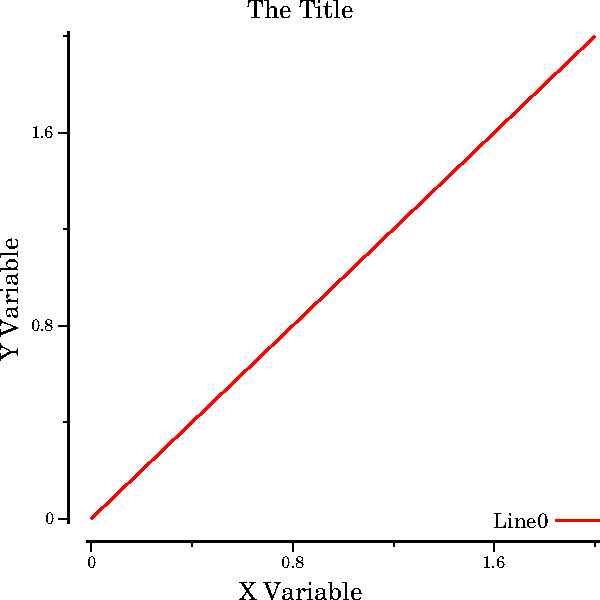
\includegraphics{simple_plot}
\caption{\label{fig:simp}A simple plot}
\end{center}
\end{figure}

\sio\ works by evaluating a plotting-expression.
Figure~\ref{fig:simp} shows the plot created from the simple
expression:

\begin{verbatim}
(output "simple_plot.pdf"
        (num-by-num-plot
         :title "The Title"
         :x-label "X Variable"
         :y-label "Y Variable"
         :legend (legend-location :lower-right)
         :dataset (line-dataset
                   :name "Line0"
                   :color (color :r 1.)
                   :points ((0 0) (1 1) (2 2)))))
\end{verbatim}

The base expression is an {\tt output} expression.  The {\tt output}
expression takes two arguments: 1) The name of the output file as a
string and 2) A plot.  The second argument to this expression is a
numeric by numeric plot (one with both numeric x and y axes).  A
numeric by numeric plot is created with the {\tt num-by-num-plot}
function (described in more detail below).  The plot in this
expression has one dataset (the red line) which is specified by the
{\tt :dataset} option to the {\tt num-by-num-plot} function.  In this
case the dataset is a line dataset that is created with the {\tt
  line-dataset} function (again described further below).

As a convenience, \sio\ has a {\tt let} or {\tt let*} expression
similar to those found in lisp or scheme.  A {\tt let} expression
allows values to be bound to a variable names.  {\tt let*} is like let
except one binding can refer to the name bound by a previous binding
in the same binding list.  Using {\tt let*}, the previous expression
could be re-written:

\begin{verbatim}
(let* ((dataset0 (line-dataset
                  :name "Line0"
                  :color (color :r 1.)
                  :points ((0 0) (1 1) (2 2))))
       (plot0 (num-by-num-plot
               :title "The Title"
               :x-label "X Variable"
               :y-label "Y Variable"
               :legend (legend-location :lower-right)
               :dataset dataset0)))
  (output "simple_plot.pdf" plot0))
\end{verbatim}

The following sections give detailed information on the functions
available in \sio.

\section{\sio\ Expressions}

The \sio\ expression language is similar to lisp or scheme (I think).
The basic types or values are:
\begin{itemize}
\item Numbers (represented as floats)
\item Strings (characters between `` '' marks)
\item Identifiers (un-quoted strings)
\item Lengths (created with the length functions described below)
\item Colors (created with the color function)
\item Legend locations (created with the legend-location function)
\item Numeric by numeric plots (Section~\ref{sect:num-by-num})
\item Numeric by numeric datasets (Section~\ref{sect:num-by-num})
\item Numeric by nominal plots (Section~\ref{sect:num-by-nom})
\item Numeric by nominal datasets (Section~\ref{sect:num-by-nom})
\item A list of values (values inbetween '(' ')').  Lists beginning
  with identifiers are functions.  All other lists are treated as
  data.
\begin{verbatim}
("a data list" 5 7 4 9 "hello" ("foo") "baz")
(this-is-a-function "because it starts with an identifier" 3 (in 5))
\end{verbatim}
\end{itemize}

\subsection{Getting Help}

The {\tt help} function can be used to get help on the available
functions in \sio.  Example:
\begin{verbatim}
> (help num-by-num-plot)
(num-by-num-plot [:title <string>] [:x-label <string>]
[:y-label <string>] [:width <length>] [:height <length>]
[:x-min <number>] [:x-max <number>] [:y-min <number>] [:y-max <number>]
[:dataset <num-by-num-dataset>]+)
Creates a plot with numeric x and y axes.
\end{verbatim}

\subsection{Lengths}

Lengths can be used to specify the size of things.  Lengths can be
specified in inches, centimeters, points or pixels using the
respective functions {\tt in}, {\tt cm}, {\tt pt} or {\tt px}.  For
example:
\begin{verbatim}
(in 5)
\end{verbatim}
creates a length of 5 inches.

\subsection{Colors}

Colors can be used to specify the color of things.  Colors are created
with the {\tt color} function.  The {\tt color} function has four
options: {\tt :r}, {\tt :g}, {\tt :b} and {\tt :a} that specify the
red, green, blue and alpha components of the color respectively.  The
default for the all options is 0 except for {\tt :a} that defaults to
1. For example:
\begin{verbatim}
(color :g 0.5 :a 0.5)
\end{verbatim}
creates a green color that is half opaque.


\subsection{Legend locations}

Legend locations are also values.  These can be used to specify the
location of the legend in a numeric by numeric plot.  The available
legend locations are:
\begin{description}
\item[{\tt :upper-right}] Upper right corner of the plot.
\item[{\tt :upper-left}] Upper left corner of the plot.
\item[{\tt :lower-right}] Lower right corner of the plot.
\item[{\tt :lower-left}] Lower left corner of the plot.
\item[{\tt (legend-at <text-placement> <number> <number>)}] Puts the
  legend at a specified location.  <text-placement> is one of: {\tt
    :text-before} or {\tt :text-after} and the numbers are the x and y
  location of the legend.
\end{description}
For example, the this location
\begin{verbatim}
(legend-location :upper-right)
\end{verbatim}
puts the legend in the upper right corner of the plot and this
location
\begin{verbatim}
(legend-location (legend-at :text-before 100 100))
\end{verbatim}
puts the legend at location 100,100 with the text before the icons.

\section{Data}

Data can be specified in-line in the spt input as lists of numbers (or
lists of lists of numbers, etc.) depending on the required format.
For example a list of points may be specified as:
\begin{verbatim}
((0 0) (1 1) (2 2))
\end{verbatim}

Sometimes it is convenient to specify data in a separate file.  A list
of numbers can be read from a file using the {\tt data-file} function.
This function takes one argument that is the name of the file to read.
In addition, it is often useful to process data as the result of
running an external program. The {\tt data-cmd} function takes a
single argument that is a command to execute with the shell.  The
standard output of the command is read as a list of numbers.
Once a list of numbers has been read, either from a file or a command,
it may be grouped into points, triples, etc. using the {\tt group}
function.  This function takes two parameters: 1) a number that
specifies the size of each group and 2) a list of numbers to group.

For example the following trace of execution was given using a file
called ``data.dat'' that contained the numbers ``0 0 1 1 2 2 3 3 4 4 5
5'':
\begin{verbatim}
> (print (data-file "data.dat") "\n")
( 0 0 1 1 2 2 3 3 4 4 5 5 )
> (print (group 2 (data-file "data.dat")) "\n")
( ( 0 0 ) ( 1 1 ) ( 2 2 ) ( 3 3 ) ( 4 4 ) ( 5 5 ) )
> (print (group 3 (data-file "data.dat")) "\n")
( ( 0 0 1 ) ( 1 2 2 ) ( 3 3 4 ) ( 4 5 5 ) )
> (print (data-cmd "cat data.dat") "\n")
( 0 0 1 1 2 2 3 3 4 4 5 5 )
> (print (group 2 (data-cmd "sed s/0/-1/g data.dat")) "\n")
( ( -1 -1 ) ( 1 1 ) ( 2 2 ) ( 3 3 ) ( 4 4 ) ( 5 5 ) )
\end{verbatim}
Notice how it is now simple to specify a list of values, points or
triples by simply reading in a file or executing a command that
results in a stream of numbers.

\section{Outputting and Displaying Plots}

\begin{description}
\item[{\tt (output <string> <plot>)}]
Output the given plot to the given
file.  The first argument is a file name string.  The extension given
in the file name dictates the output file format.  The format can be
any one supported by {\tt spt}: .pdf, .ps or .png.  The second
argument is a plot expression.

\item [{\tt (display <plot>)}] Displays the given plot using GTK.
\end{description}

\section{Functions with Option Lists}

Some functions take their arguments as options lists in the form: {\tt
  [<option> <value>]*} where {\tt <option>} is an identifier beginning
with a ``:'' and {\tt <value>} is an expression that is the value of
the given option.  The simple plot in Figure~\ref{fig:simp} is created
using the {\tt num-by-num-plot} and {\tt line-dataset} functions.
Both of these are examples of functions that use option lists.

\section{\label{sect:num-by-num} Numeric by Numeric Plots}

Numeric by numeric plots are standard plots with numeric x and y axes.
These plots are created using the {\tt num-by-num-plot} function.  The
{\tt num-by-num-plot} function has the following options:

\begin{center}
\begin{tabular}{lll}
Option & Default & Notes \\
\hline
:title & & Plot title text\\
:x-label & & X label text\\
:y-label & & Y label text\\
:width & 4in & The width of the plot\\
:height & 4in & The height of the plot\\
:x-min & & The minimum x-axis value\\
:x-max & & The maximum x-axis value\\
:y-min & & The minimum y-axis value\\
:y-max & & The maximum y-axis value\\
:sort-legend & true & Whether or not to sort the legend on the mean y
value \\
:legend & :upper-right & The location of the legend \\
:dataset & & A dataset to add to the plot.  (See below for available
datasets).\\
\end{tabular}
\end{center}

\subsection{Numeric by Numeric Datasets}

The following are the available numeric by numeric datasets:

\subsubsection{\tt scatter-dataset}

Makes a dataset that displays a glyph at each of the given points.

\begin{center}
\begin{tabular}{lll}
Option & Default & Notes \\
\hline
:name & & The name, if not specified the dataset doesn't show in
the legend\\
:glyph & & ``circle'', ``ring'', ``cross'', ``plus'', ``square'',
``box'', ``triangle'' or string of len1\\
:color & & The color of the glyphs\\
:point-radius & 4pt & The radius of the glyphs\\
:points & & The data points as a list of 2-lists of numbers\\
\end{tabular}
\end{center}

If {\tt :glyph} is not specified then the next glyph is used in a
default list of glyphs.

Note: if more than one {\tt :points} options are specified the
behavior is to concatenate the points into one single list of points.

\subsubsection{\tt scatter-errbar-dataset}

Makes a dataset that displays a glyph at the median of a cluster of
points along with a 90\% confidence interval on both the x and y
values.

\begin{center}
\begin{tabular}{lll}
Option & Default & Notes \\
\hline
:name & & The name, if not specified the dataset doesn't show in
the legend\\
:glyph & & ``circle'', ``ring'', ``cross'', ``plus'', ``square'',
``box'', ``triangle'' or string of len1\\
:color & & The color of the glyphs\\
:point-radius & 4pt & The radius of the glyphs\\
:cluster & & A list of points optionally preceded by a string.
\end{tabular}
\end{center}

If {\tt :glyph} is not specified then the next glyph is used in a
default list of glyphs.

Note: if more than one {\tt :points} options are specified the
behavior is to concatenate the points into one single list of points.

\subsubsection{\tt bestfit-dataset}

Makes a dataset that displays a glyph at each of the given points with
a best polynomial fit.  The options are the same as for {\tt
  scatter-dataset} except the following additional option is
available.

\begin{center}
\begin{tabular}{lll}
Option & Default & Notes \\
\hline
:dashes & & A list of lengths {\tt (<on> <off> ...)} that specify the
dash pattern of the line\\
:degree & 1 & The degree of the polynomial to fit. \\
:fit-in-name & true & If true, the best fit function is added to the end
of the dataset name.\\
\end{tabular}
\end{center}

If {\tt :dashes} is not specified then the next in a default list of
dash patterns is used.

\subsubsection{\tt bubble-dataset}

Creates a bubble plot.  This is like a scatter plot but the data is
specified in triples {\tt (<i> <j> <k>)} where the first and second
value are the x and y coordinates of the bubble and the third value is
used to specify the size of the bubble.  The options are the same as
for {\tt scatter-dataset} except instead of {\tt :point-radius} the
minimum and maximum radius are given and the data is given in triples
instead of points:

\begin{center}
\begin{tabular}{lll}
Option & Default & Notes \\
\hline
:min-radius & 10pt & The minimum radius of a bubble\\
:max-radius & 60pt & The maximum radius of a bubble\\
:triples & & The data as a list of 3-lists of numbers\\
\end{tabular}
\end{center}

\subsubsection{\tt line-dataset}

A line dataset.  This draws a simple line.

\begin{center}
\begin{tabular}{lll}
Option & Default & Notes \\
\hline
:name & & The name, if not specified the dataset doesn't show in
the legend\\
:dashes & & A list of lengths {\tt (<on> <off> ...)} that specify the
dash pattern of the line\\
:color & & The color of the line\\
:line-width & 1pt & The width of the line\\
:points & & The data points\\
\end{tabular}
\end{center}

If {\tt :dashes} is not specified then the next in a default list of
dash patterns is used.

\subsubsection{\tt line-points-dataset}

A line with glyphs drawn at each point.  This dataset has the same
options as {\tt scatter-dataset} and {\tt line-dataset}.

\subsubsection{\tt line-errbar-dataset}

This dataset is given a set of lines.  The plot shows the interpolated
mean value line with error bars showing a 95\% confidence interval.

\begin{center}
\begin{tabular}{lll}
Option & Default & Notes \\
\hline
:name & & The name, if not specified the dataset doesn't show in
the legend\\
:dashes & & A list of lengths {\tt (<on> <off> ...)} that specify the
dash pattern of the line\\
:color & & The color of the line\\
:line-width & 1pt & The width of the line\\
:lines & & A list of lists of 2-lists of numbers.  Each list of
2-lists is a line (x-sorted)\\
\end{tabular}
\end{center}

As an example, the following expression will create the plot shown in
Figure~\ref{fig:line_err}:

\begin{verbatim}
(let* ((line0 ((0 0) (1 1) (2 2)))
       (line1 ((0 -1) (1 0) (2 1)))
       (line2 ((0 1) (1 2) (2 3)))
       (dataset0 (line-errbar-dataset
                  :name "Line with errar bars"
                  :lines (line0 line1 line2)))
       (plot0 (num-by-num-plot
               :legend (legend-location :lower-right)
               :dataset dataset0)))
  (output "line_err.pdf" plot0))
\end{verbatim}

\begin{figure}[t]
\begin{center}
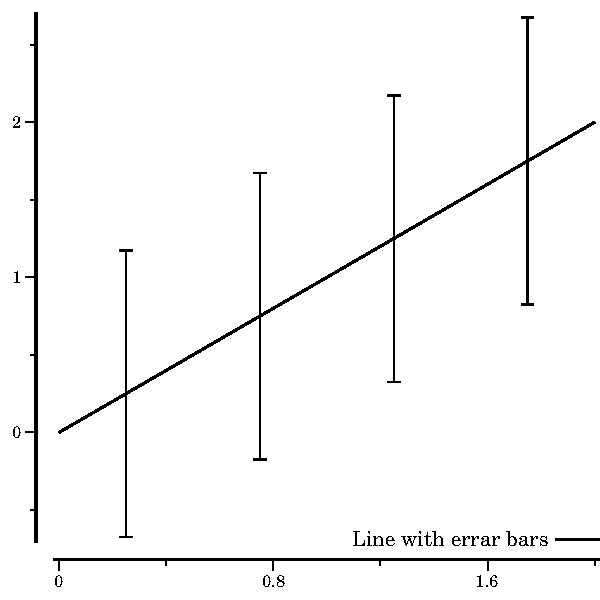
\includegraphics{line_err}
\caption{\label{fig:line_err}A mean-line with error bars plot.}
\end{center}
\end{figure}

\subsubsection{\tt histogram-dataset}

A histogram shows a distribution of values.

\begin{center}
\begin{tabular}{lll}
Option & Default & Notes \\
\hline
:name & & The name, if not specified the dataset doesn't show in
the legend\\
:dashes & & A list of lengths {\tt (<on> <off> ...)} that specify the
dash pattern of the line\\
:color & & The color of the line\\
:line-width & 1pt & The width of the line\\
:bin-width &  & The width each bin\\
:values & & A list of values (each represent a weight of 1) \\
:points & & A list of points (x=value, y=weight)\\
\end{tabular}
\end{center}

The default bin-width creates $\sqrt{n}$ bins where $n$ is the number
of data values.  {\tt :line-width} and {\tt :dashes} control the look
of the line forming the bars of the histogram.

\subsubsection{\tt cdf-dataset}

A histogram shows a cumulative distribution of values.
The options are the same as for a histogram except that there is no
{\tt :bin-width} option.

\subsubsection{\tt heatmap-dataset}

A heatmap is a grid of colored x, y cells.  The z values that fall
within each cell are summed to compute the color.

\begin{center}
\begin{tabular}{lll}
Option & Default & Notes \\
\hline
:bin-size & & An (x, y) point specifying the size of each cell.\\
:triples & & A list of triples (x, y, z)\\
\end{tabular}
\end{center}

\subsubsection{\tt num-by-num-composite}

New datasets can be created by putting other datasets together.  For
example, the following expression will create a step function shown in
Figure~\ref{fig:step} by compositing three line datasets:

\begin{verbatim}
(let* ((line0 ((0 0) (1 0)))
       (line1 ((1 1) (2 1)))
       (line2 ((2 2) (3 2)))
       (line-ds0 (line-dataset :dashes () :points line0))
       (line-ds1 (line-dataset :dashes () :points line1))
       (line-ds2 (line-dataset :dashes () :points line2))
       (dataset0 (num-by-num-composite
                  :name "Step function"
                  :dataset line-ds0
                  :dataset line-ds1
                  :dataset line-ds2))
       (plot0 (num-by-num-plot
               :legend (legend-location :lower-right)
               :dataset dataset0)))
  (output "step_func.pdf" plot0))
\end{verbatim}

\begin{figure}[t]
\begin{center}
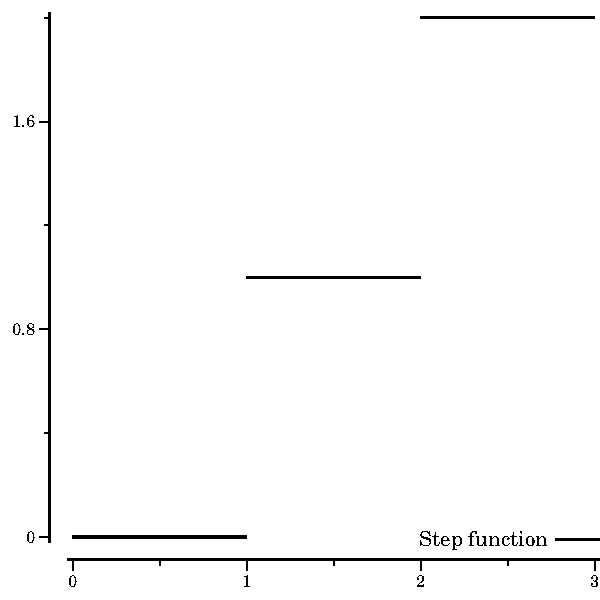
\includegraphics{step_func}
\caption{\label{fig:step}A simple step-function.}
\end{center}
\end{figure}

\section{\label{sect:num-by-nom} Numeric by Nominal Plots}

Numeric by nominal plots are plots with an numeric y-axis but a
nominal x axis.  In this type if plot, each dataset is allocated a
fixed width of the x axis into which it will be displayed.  These
types of plots are created using the {\tt num-by-nom-plot} function
that takes the following options:


\begin{center}
\begin{tabular}{lll}
Option & Default & Notes \\
\hline
:title & & Plot title text\\
:y-label & & Y label text\\
:width & 4in & The width of the plot\\
:height & 4in & The height of the plot\\
:y-min & & The minimum y-axis value\\
:y-max & & The maximum y-axis value\\
:horiz-line & & The y-value of an optional horizontal line\\
:dataset & & A dataset to add to the plot.  (See below for available
datasets).\\
\end{tabular}
\end{center}

\subsection{Numeric by Nominal Datasets}

The following are the available numeric by nominal datasets:

\subsubsection{\tt boxplot-dataset}

Makes a boxplot dataset.

\begin{center}
\begin{tabular}{lll}
Option & Default & Notes \\
\hline
:name & & The name (required)\\
:point-radius & 2pt & The radius of the glyphs\\
:values & & The data values as a list of numbers\\
\end{tabular}
\end{center}

\subsubsection{\tt barchart-dataset}

Makes a single bar for a barchart.

\begin{center}
\begin{tabular}{lll}
Option & Default & Notes \\
\hline
:name & & The name (required)\\
:value & & The data value as a number\\
\end{tabular}
\end{center}

\subsubsection{\tt barchart-errbar-dataset}

Makes a single bar for a barchart where the height of the bar is the
mean of a set of values and an error bar shows the 95\% confidence
interval.

\begin{center}
\begin{tabular}{lll}
Option & Default & Notes \\
\hline
:name & & The name (required)\\
:values & & The data values as a list of numbers\\
\end{tabular}
\end{center}

\subsubsection{\tt num-by-nom-group}

Groups a set of numeric by nominal datasets.  This will draw an
over-bar above the names of the datasets in the group and an optional
group name centered beneath the names in the group.

\begin{center}
\begin{tabular}{lll}
Option & Default & Notes \\
\hline
:name & & The name\\
:dataset & & A data set to group\\
\end{tabular}
\end{center}

For example, the following expression creates a numeric by nominal
plot with two groups, one of boxplots and one of bar charts with error
bars shown in Figure~\ref{fig:num_by_nom}:
\begin{verbatim}
(let* ((values0 (0 0 1 1 2 2 3 3 4 4 5 5))
       (group-0-0 (boxplot-dataset :name "box0" :values values0))
       (group-0-1 (boxplot-dataset :name "box1" :values values0))
       (group-0-2 (boxplot-dataset :name "box2" :values values0))
       (group-1-0 (barchart-errbar-dataset :name "box0" :values values0))
       (group-1-1 (barchart-errbar-dataset :name "box1" :values values0))
       (group-1-2 (barchart-errbar-dataset :name "box2" :values values0))
       (dataset0 (num-by-nom-group :name "group0"
                                   :dataset group-0-0
                                   :dataset group-0-1
                                   :dataset group-0-2))
       (dataset1 (num-by-nom-group :name "group1"
                                   :dataset group-1-0
                                   :dataset group-1-1
                                   :dataset group-1-2))
       (plot0 (num-by-nom-plot :dataset dataset0 :dataset dataset1)))
  (output "num_by_nom.pdf" plot0))
\end{verbatim}

\begin{figure}[t]
\begin{center}
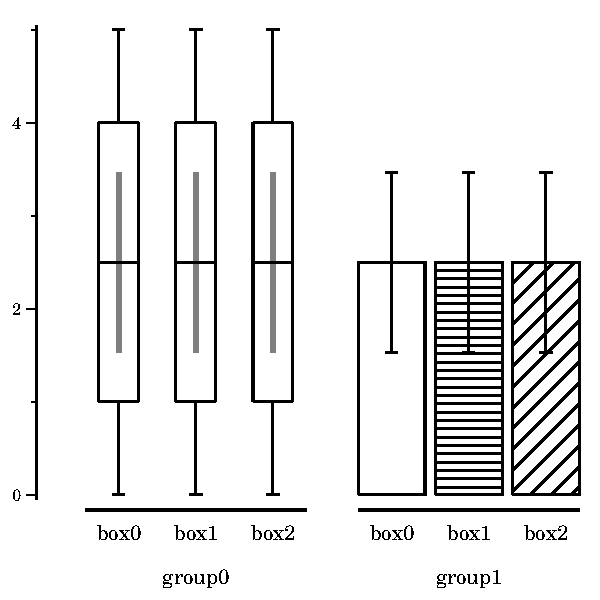
\includegraphics{num_by_nom}
\caption{\label{fig:num_by_nom}A numeric by nominal plot with groups.}
\end{center}
\end{figure}

\end{document}
